\documentclass[a4paper,10pt]{article}
\usepackage[utf8]{inputenc}
\usepackage{graphicx}
%opening
\title{Offensive Security\\Lab-report 4}
\author{Moritz Rupp}

\begin{document}

\maketitle


\newpage
\section{Lab 4}
\subsection{A Basic Stack Overflow Attack}
We are provided with a vulnareble piece of C Code that can be exploited to trigger a basic Stack overflow. Since modern architectures have several countermeasures to prevent such abuse, we have to compile the Code as shown in the lecture nodes to let the exploit work!
\begin{center}
 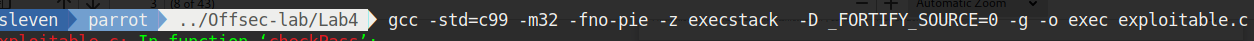
\includegraphics[scale=0.3]{gcc.png}
\end{center} 
After failing to trigger the exploit by simply passing different input lengths, we take a closer look at the programm with the help of GDB.\\
At first we look at the assemler Code. To make it more readable we set the disassembler flavor to intel. 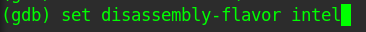
\includegraphics[scale=0.4]{intelfalvor.png}\\
After further inspection we realize that we need to find the starting adress of the hidden function.
\begin{center}
 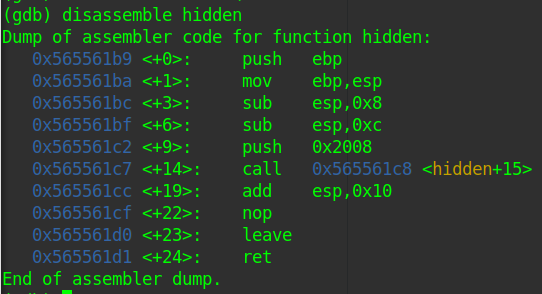
\includegraphics[scale=0.5]{hidden.png}
\end{center}
Starting adress is '0x565561b9'.\\
When we pass this adress to eip we can execute the function 'hidden'.
With the help of breakpoints and single stepping we reckon to overwrite 16bytes.
Hence we write 16 arbitrary bytes followed by the starting adress of the hidden function to a file and pipe it to the binary execution. 
\begin{center}
 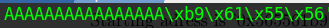
\includegraphics[scale=0.5]{bytes.png}
\end{center}
This doesnt work and after some research, we find this is due to different architecture design(e.g. adding random byte lengths to registers). When we add 4 more bytes it works!
\begin{center}
 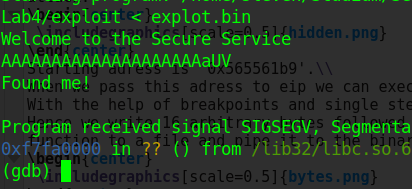
\includegraphics[scale=0.5]{found.png}
\end{center}
\subsection{Spawning A Shell With Shellcode}
This time we want to inject our own code to spawn a shell by executing 'bin/bash'. We are provided with a similar C programm that expects an input parameter this time, but has the same vulnerability. We want to inject the string of 'bin/bash' to the stack and then execute the 'command' with the help of a system call.
We construct this by writing a simple assembler 'programm' and compile it with the help of nasm. This results in a file with the corresponding object code that includes the shellcode as an hexadecimal string which we can pass to the programm with perl. 
Furthermore we have to determine the adress of buff and add it to the input.
\begin{center}
 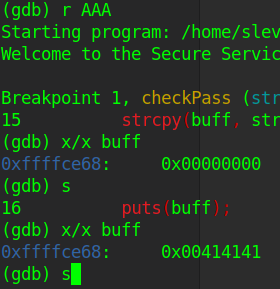
\includegraphics[scale=0.5]{breakpoint.png}
\end{center}
Buff has 0xffffce68. Adding up 8 bytes of dummy data to fill buff plus overwriting the stack pointer and the return adress we need to pass 16 bytes before we can deliver our payload.\\
This results in the following input parameter.
When we feed this to the programm we spawn a shell.


\newpage
\subsection{}
\end{document}
